\documentclass[sigconf]{acmart}

\usepackage{color}
\usepackage{balance}
\usepackage{blindtext}
\usepackage{comment}
\usepackage{amsmath}
\usepackage{enumitem}
\usepackage{array}
\usepackage{graphicx}
\usepackage{subcaption}
\usepackage{tabularx}
\usepackage{ragged2e}
\usepackage{adjustbox}
\usepackage{multirow}
\usepackage{booktabs}
\usepackage{caption}
\usepackage{float}
\usepackage{url}
\usepackage{xspace}
\usepackage[newfloat]{minted}
\usepackage[english]{babel}



\newenvironment{code}{\captionsetup{type=listing}}{}
\SetupFloatingEnvironment{listing}{name=Listing}
\newcolumntype{P}[1]{>{\centering\arraybackslash}m{#1}}

% Copyright
\setcopyright{none}
%\setcopyright{acmcopyright}
%\setcopyright{acmlicensed}
% \setcopyright{rightsretained}
%\setcopyright{usgov}
%\setcopyright{usgovmixed}
%\setcopyright{cagov}
%\setcopyright{cagovmixed}

\setlength{\textfloatsep}{5pt}
\setlength{\intextsep}{5pt}
\newcommand{\namex}{\mbox{\sf Compass}}
\newcommand{\name}{\namex\xspace}
\newcommand{\Paragraph}[1]{~\vspace*{-0.8\baselineskip}\\{\bf #1}}
\DeclareMathOperator{\sen}{sen}
\newcommand{\Q}{\mathbb{Q}}
\newcommand{\alphastar}{\alpha^{*}}
\newcommand{\blue}[1]{{\color{blue} #1}}

\newcommand{\cb}[1]{{\color{blue} #1}}

%\newtheorem{definition}{Definition}
%\newtheorem{theorem}{Theorem}
%%\newtheorem{proof}{Proof}
%\newtheorem{lemma}{Lemma}
%\newtheorem{corollary}{Corollary}

\newcommand\Tstrut{\rule{0pt}{2.6ex}}       % "top" strut
\newcommand\Bstrut{\rule[-0.9ex]{0pt}{0pt}} % "bottom" strut
\newcommand{\TBstrut}{\Tstrut\Bstrut} % top&bottom struts

%\renewcommand{\algorithmicrequire}{\textbf{Input:}}
%\renewcommand{\algorithmicensure}{\textbf{Output:}}
\newcommand\floor[1]{\lfloor#1\rfloor}
\newcommand\ceil[1]{\lceil#1\rceil}
\newcommand\F{\widehat{F}}
\newcommand\be{\widehat{b}}

\newcommand{\pbex}{\mbox{\sf PBE}}
\newcommand{\pbe}{\pbex\xspace}
\newcommand{\pbeaX}{\mbox{\sf PBE-1}}
\newcommand{\pbea}{\pbeaX\xspace}
\newcommand{\pbebX}{\mbox{\sf PBE-2}}
\newcommand{\pbeb}{\pbebX\xspace}
\newcommand{\cmpbeaX}{\mbox{\sf CM-PBE-1}}
\newcommand{\cmpbea}{\cmpbeaX\xspace}
\newcommand{\cmpbebX}{\mbox{\sf CM-PBE-2}}
\newcommand{\cmpbeb}{\cmpbebX\xspace}
\newcommand{\cmpbex}{\mbox{\sf CM-PBE}}
\newcommand{\cmpbe}{\cmpbex\xspace}
\newcommand{\eps}{\varepsilon}


\newtheorem{informal}{Informal Problem}
\newtheorem*{formal}{Open Attribute Value Extraction}
\newcommand{\sysname}{{\sf OpenTag}\xspace}
%\newcommand{\softmax}{\operatornamewithlimits{softmax}}
%\newcommand{\argmax}{\operatornamewithlimits{argmax}}
\DeclareMathOperator{\softmax}{softmax}
\DeclareMathOperator{\argmax}{argmax}
\DeclareMathOperator{\argmin}{argmin}
\pagenumbering{arabic}
\setcounter{page}{1}

\newenvironment{pkl}{%
\begin{itemize}%
%\vspace{-\topsep}%
\setlength\itemsep{-0.5\parskip}%
\setlength\parsep{0in}%
}{%
%\vspace{-\topsep}%
\end{itemize}}

\newenvironment{des}{%
\begin{description}%
%\vspace{-\topsep}%
\setlength\itemsep{-0.5\parskip}%
\setlength\parsep{0in}%
}{%
%\vspace{-\topsep}%
\end{description}}


\newenvironment{enu}{%
\begin{enumerate}%
\vspace{-\topsep}%
\setlength\itemsep{-\parskip}%
\setlength\parsep{0in}%
}{%
\vspace{-\topsep}%
\end{enumerate}}



%Conference

\copyrightyear{2018}
\acmYear{2018}
%\setcopyright{none}
\acmConference{University of Utah}{}{ Salt Lake City, USA.}
%\acmPrice{15.00}
%\acmISBN{-}
%\acmDOI{-}


\setlength{\textfloatsep}{1pt}
\setlength{\intextsep}{7pt}
\setlength{\floatsep}{3pt}

\begin{document}
\title{ Spatio-temporal Public Health Analysis and its Ethical Concerns}
% \titlenote{Produces the permission block, and
%   copyright information}
%\subtitle{}
%\subtitlenote{The full version of the author's guide is available as
%  \texttt{acmart.pdf} document}

\author{Debjyoti Paul}
\affiliation{%
    \institution{University of Utah}
}
\email{deb@cs.utah.edu}




% The default list of authors is too long for headers}
%\renewcommand{\shortauthors}{B. Trovato et al.}

% \begin{abstract}

\end{abstract}


%
% The code below should be generated by the tool at
% http://dl.acm.org/ccs.cfm
% Please copy and paste the code instead of the example below.
%
%\begin{CCSXML}
%<ccs2012>
% <concept>
%  <concept_id>10010520.10010553.10010562</concept_id>
%  <concept_desc>Computer systems organization~Embedded systems</concept_desc>
%  <concept_significance>500</concept_significance>
% </concept>
% <concept>
%  <concept_id>10010520.10010575.10010755</concept_id>
%  <concept_desc>Computer systems organization~Redundancy</concept_desc>
%  <concept_significance>300</concept_significance>
% </concept>
% <concept>
%  <concept_id>10010520.10010553.10010554</concept_id>
%  <concept_desc>Computer systems organization~Robotics</concept_desc>
%  <concept_significance>100</concept_significance>
% </concept>
% <concept>
%  <concept_id>10003033.10003083.10003095</concept_id>
%  <concept_desc>Networks~Network reliability</concept_desc>
%  <concept_significance>100</concept_significance>
% </concept>
%</ccs2012>
%\end{CCSXML}
%
%\ccsdesc[500]{Computer systems organization~Embedded systems}
%\ccsdesc[300]{Computer systems organization~Redundancy}
%\ccsdesc{Computer systems organization~Robotics}
%\ccsdesc[100]{Networks~Network reliability}
%
% We no longer use \terms command
%\terms{Theory}

%\keywords{ streaming data, bursty, data sketch, historical queries}


\maketitle

% \begin{abstract}

\end{abstract}

\section*{Overview}
\label{sec:overview}
The term {\em Social Media} gained widespread attention with the advent of Web 2.0 in the first decade of 20th century \cite{kaplan2010users}. Web 2.0 is also known as {\em participative} or {\em social web} that emphasize on user interaction and user generated content encouraging participatory culture. Before we jump into more details of social media, it would be wiser to define it.
The dynamic changes and continuous development of social media services makes it harder to define them, however most of the research work could be summarized it as follows.

\begin{definition}[Social Media]
Social media is an interactive computer mediated technological platform that facilitates the creation and sharing of information, ideas, career interests and other forms of expression via virtual communities and networks \cite{kietzmann2011social}.
\end{definition}

In contrast to the {\em traditional media} which operates under a monologic transmission model i.e. one source to many receivers, such as a television, newspaper  or a radio station which broadcasts the same programs to an entire city; {\em social media} are dialogic transmission system which brings interaction, usability and a notion of individual entity in the digital world.




%%% Local Variables:
%%% mode: latex
%%% TeX-master: "main"
%%% End:

\section{Part A}
\label{part_a}
In reinforcement learning there is no supervisor but a {\em reward} signal to guide the learning process. Even the feedback is delayed and not instantaneous which sets it as a different paradigm from other machine learning methods. In a sequential decision making process an/the {\em agent} gets to pick an action at every time step which tries to optimize the future cumulative {\em reward} signal.
Traditional Reinforcement Learning
requires explicit design of state space and action space, while the mapping from state space to action space is learned \cite{sutton1998introduction}.
 That makes the problem spaces and the possible states in an environment very limited, only with fully observable state of environment for agent.  Neural networks enhances RL with the capability to make the agent learn a state abstraction and a policy approximation directly from its input data in a partially observable environment. Deep RL is the fruitful outcome of this attempt of RL enhancement.

\subsection{Formal RL Framework:}
\label{formal_rl}
The general RL problem is formalized as a discrete time stochastic
control process where an agent interacts with its environment in the
following way: the agent starts, in a given state within its environment
$s_0 \in \mathcal{S}$, by gathering an initial observation $\omega_0 \in \Omega$. At each time
step $t$, the agent has to take an action $a_t \in \mathcal{A}$. As illustrated in
Figure \ref{fig:rl_01} it follows three consequences: (i) the agent obtains a reward
$r_t \in \mathcal{R}$, (ii) the state transitions to $s_{t+1} \in \mathcal{S}$, and (iii) the agent obtains
an observation $\omega_{t+1} \in \Omega$. This control setting was first proposed by
\cite{bellman1957dynamic} and later extended to learning by Barto \cite{barto1983neuronlike}.
The goal of RL is to {\em select actions to maximise total future reward}.
\begin{figure}[t]
	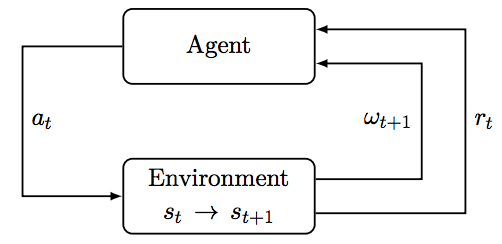
\includegraphics[width=0.7\linewidth ]{fig/agent.png}
    \vspace{-2mm}
    \caption{Agent-environment interaction in RL.}
    \label{fig:rl_01}
\end{figure}

\definition{\em Reward:}
A reward $r_t$ is a scalar feedback signal that indicates how well {\em agent} is doing at step $t$.

An example of  {\em reward} in the case of flying toy robot helicopters are : (a) $+$ve reward for following desired trajectory, (b) $−$ve reward for crashing.

\definition{\em History:} The history $\mathcal{H}_t$ is the sequence of observations, actions, rewards, i.e. all observable variables up to time $t$. Mathematically, $\mathcal{H}_t = \omega_1,r_1,a_1,\ldots,a_{t-1},\omega_t,r_t$.

Formally, state $s_t \in \mathcal{S}$ is a function of the history $\mathcal{H}_t$.
$$s_t = f(\mathcal{H}_t)$$

Environment and agent both can have their own state which we define as $s_t^e$ and $s_t^a$ respectively. The environment state is usually not visible to the agent.

In a fully observable system, the agent directly observes environment state i.e. $\omega_t = s^a_t = s_t^e$. Formally this is called as Markov Decision Process (MDP). The Markov property means that the future of the process only
depends on the current observation and the agent has no interest in
looking at the full history.

\Paragraph{Markov Decision Process (MDP):}\\  An MDP is a 5-tuple $(\mathcal{S}, \mathcal{A}, T, \mathcal{R}, \gamma)$ where
\begin{itemize}
  \item[] $\mathcal{S}$ is the state space,
  \item[] $\mathcal{A}$ is the action space,
  \item[] $T : \mathcal{S} \times \mathcal{A}\times \mathcal{S} \rightarrow [0, 1]$ is the transition function (set of conditional
  transition probabilities between states),
  \item[] R: $\mathcal{S} \times \mathcal{A}\times \mathcal{S} \rightarrow \mathcal{R}$ is the reward function, where $R$ is a continuous set of possible rewards in a range $R_{max} \in \mathbb{R}^+$ (e.g., $[0, R_{max}]$),
  \item[] $\gamma \in  [0, 1)$ is the discount factor.
\end{itemize}

% $\mathcal{A}$ is the action space, \\
% $T : \mathcal{S} \times \mathcal{A}\times \mathcal{S} \rightarrow [0, 1]$ is the transition function (set of conditional
% transition probabilities between states), \\
% R: $\mathcal{S} \times \mathcal{A}\times \mathcal{S} \rightarrow \mathcal{R}$ is the reward function, where $R$ is a continuous set of possible rewards in a range $R_{max} \in \mathbb{R}^+$ (e.g., $[0, R_{max}]$), \\
% $\gamma \in  [0, 1)$ is the discount factor.

\vspace{3mm}

However, in the real world not many systems are fully observable, an {\em agent} indirectly observes the environment without knowing it's internal information state. In this scenario $s_t^a \neq s^e_t$.



Formally this is a partially observable Markov decision process (POMDP) illustrated in Figure \ref{fig:pomdp}.
\vspace{5mm}
\Paragraph{Partially Observable Markov Decision Process (POMDP):}
A POMDP is a 7-tuple $(\mathcal{S}, \mathcal{A}, T, \mathcal{R}, \Omega, O, \gamma)$ where
\begin{itemize}
  \item[] $\mathcal{S}$ is the state space,
  \item[] $\mathcal{A}$ is the action space,
  \item[] $T : \mathcal{S} \times \mathcal{A}\times \mathcal{S} \rightarrow [0, 1]$ is the transition function (set of conditional
  transition probabilities between states),
  \item[] R: $\mathcal{S} \times \mathcal{A}\times \mathcal{S} \rightarrow \mathcal{R}$ is the reward function, where $R$ is a continuous set of possible rewards in a range $R_{max} \in \mathbb{R}^+$ (e.g., $[0, R_{max}]$),
  \item[] $\Omega$ is a finite set of observations ${1, . . . , N_{\Omega}}$,
  \item[] $O : \mathcal{S} \times \Omega \rightarrow [0, 1]$ is a set of conditional observation probabilities,
  \item[] $\gamma \in  [0, 1)$ is the discount factor.
\end{itemize}


In a POMDP {\em agent} must construct its own state representation $s_t^a$. For example,\\
(i) \textbf{Complete history:} $s_t^a = \mathcal{H}_t$.\\
(ii) \textbf{{\em Beliefs} of environment state:} $s_t^a = \mathbb{P}[s_t^e = s^1],\ldots,\mathbb{P}[s_t^e = s^n]$ where $s^k$ represents a state in environment.\\
(iii) \textbf{Recurrent Neural Network (RNN)}: $s_t^a = \sigma(s_{t-1}^a W_s + \omega_t W_o)$ where $W_s$ and $W_o$ represents weight vectors and $\sigma$ some non linear function. \cite{wierstra2010recurrent, hausknecht2015deep, heess2015memory}.

\begin{figure}[t]
	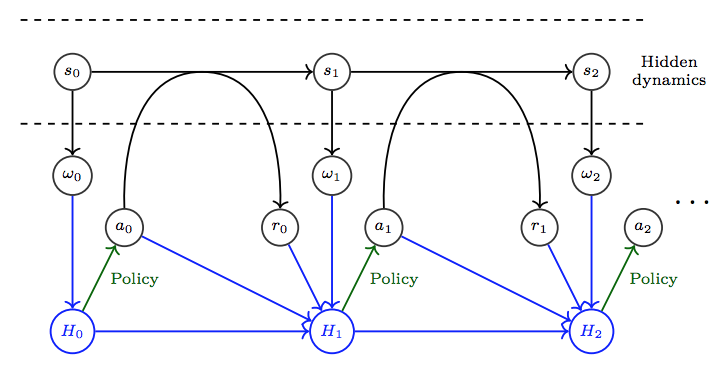
\includegraphics[width=0.9\linewidth ]{fig/pomdp.png}
    \vspace{-2mm}
    \caption{Partial Observed Markov Decision Process (POMDP).}
    \label{fig:pomdp}
\end{figure}

This RNN approach to solving
POMDPs is related to other problems using dynamical systems
and state space models, where the true state can only be
estimated \cite{bertsekas2005dynamic}.


\subsection{RL Agent Components:}
So far, we have introduced the key formalism used in RL,
the MDP and the POMDP. Now I will talk about what is inside an RL agent and the components it uses for learning. An RL agent may include one or more of the following component for learning.\\
\Paragraph{\em Value functions:}
Value function attempts to measure goodness/badness of each state and/or action.
In other words, value function methods are based on estimating the value
(expected return) of being in a given state i.e. future reward.
The state-value
function $V_{\pi}(s)$
 is the expected return when starting in state $s$
and following $\pi$ henceforth:
$$V_{\pi}(s) = \mathbb{E}_\pi [R_t +\gamma R_{t+1} + \gamma^2 R_{t+2}+\ldots  | s_t =s ]$$
where $\gamma \in [0,1]$ is a discount parameter, that governs the future sightedness of the model.
\\
\Paragraph{\em Policy Search:}  A policy is the {\em agent}'s behavior. It is a map from state to action. Examples of some policies are: \\
(i) {\em Deterministic Policy:} This is the simplest policy, here an action $a$ is mapped to a state $s$ i.e. $a = \pi(s)$.\\
(ii) {\em Stochastic Policy:} A policy can be stochastic based on probability of state observation, i.e. $\pi(a|s) = \mathbb{P}[\mathcal{A}=a |  \mathcal{S} = s]$.\\
(iii) {\em Parameterized Policy:} A parameterised policy $\pi_\theta$ is chosen, whose
parameters are updated to maximise the expected return $E[R|\theta]$ using either gradient-based or gradient-free optimisation \cite{deisenroth2013survey}. Neural networks that encode policies have been successfully
trained using both gradient-free \cite{gomez2005evolving, cuccu2011intrinsically, koutnik2013evolving} and gradient based \cite{williams1992simple, lillicrap2015continuous, heess2015learning} methods.

\Paragraph{\em Model:}
A model tries to learn the behavior of the environment. First, it tries to predict what the environment will do next, that is predicting next state and is called Transitions ($\mathcal{P}$). Secondly, the model tries to predict the expected next reward and is called Rewards model ($\mathcal{R}$).
$$\mathcal{P}^a_{ss'} = \mathbb{P}[\mathcal{S}' =s'| \mathcal{S}=s, \mathcal{A} =a]$$
where $s$ is the state prior state and $s'$ is the resultant state on action $a$.
$$\mathcal{R}^a_s = \mathbb{E}[r|\mathcal{S}=s,\mathcal{A}=a]$$
where $s$ is the state prior state and $r$ is the reward for next step on action $a$.

\subsection{RL Agent Taxonomy:}
Model methods are optional in RL systems. In fact there are many model free based methods applied for real world problems. To understand a comprehensive taxonomies of categorizing RL Agent we present it in Figure \ref{fig:taxonomy}.

\begin{figure}[t]
	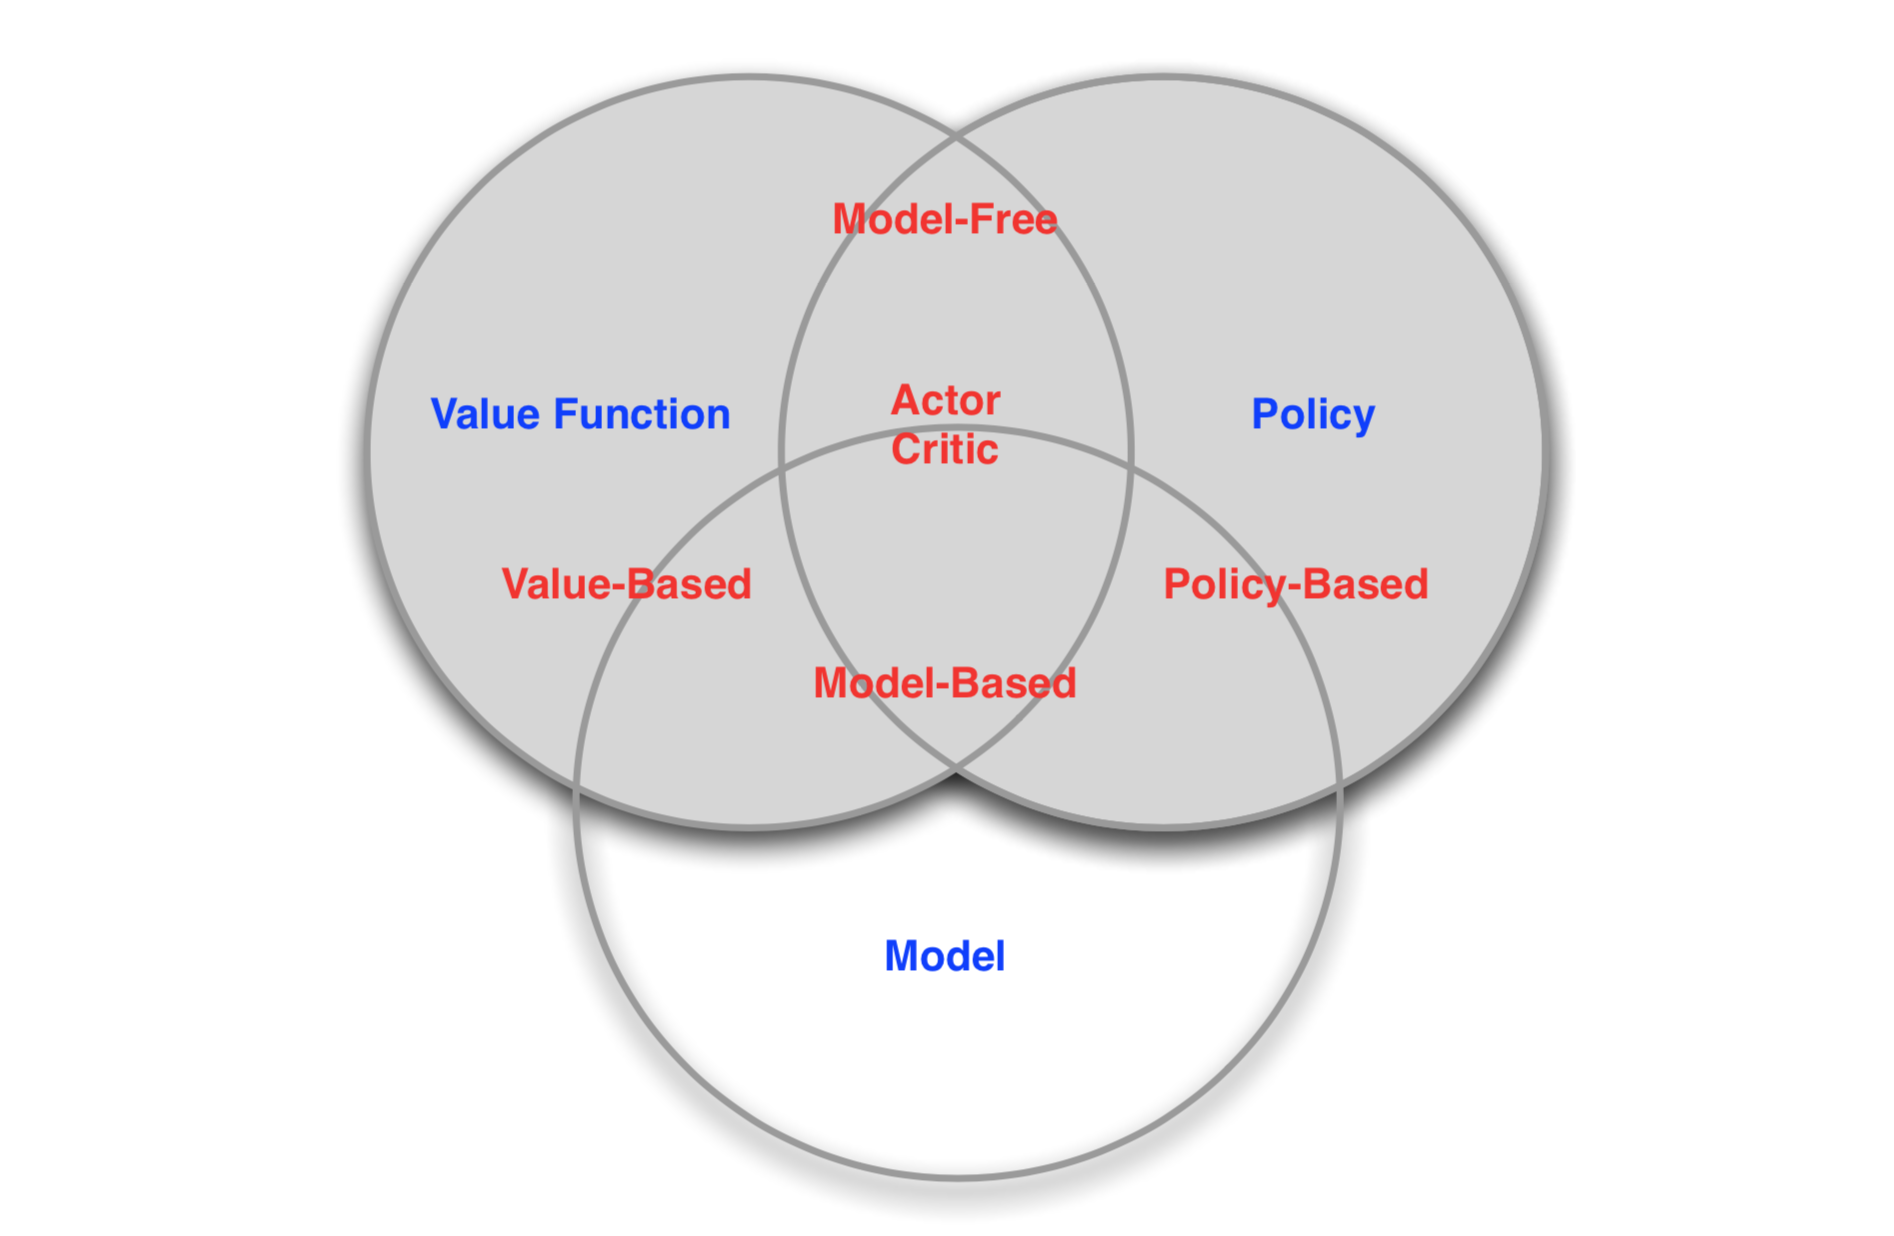
\includegraphics[width=0.7\linewidth ]{fig/taxonomy.png}
    \vspace{-2mm}
    \caption{RL Agent Taxonomy.}
    \label{fig:taxonomy}
\end{figure}

RL focus on learning without access to the underlying
model of the environment. However, interactions with the
environment could be used to learn value functions, policies,
and also a model. Model-free RL methods learn directly
from interactions with the environment, but model-based RL
methods can simulate transitions using the learned model,
resulting in increased sample efficiency \cite{arulkumaran2017brief}. This is particularly
important in domains where each interaction with the environment
is expensive. However, learning a model introduces extra
complexities, and there is always the danger of suffering from
model errors, which in turn affects the learned policy; a common
but partial solution in this latter scenario is to use model
predictive control, where planning is repeated after small
sequences of actions in the real environment \cite{bertsekas2005dynamic}.
Although
deep neural networks can potentially produce a very complex
and rich models \cite{oh2015action, finn2016deep}, sometimes simpler, more data efficient
methods are preferable \cite{gu2016continuous}.

\subsection{Deep Reinforcement Learning (DRL):}
Traditional RL works was mainly on low dimensional problems (i.e. few state space, limited actions etc.). Integration of deep neural network with RL framework bolster the framework by converting higher dimensional problems into low dimensional representations. Initial DRL works was mainly involved on scaling up prior work in RL to high dimensional problems.
DRL can deal
efficiently with the curse of dimensionality unlike tabular and
traditional non-parametric methods \cite{bengio2013representation}.

In DRL, deep neural network is trained to model/predict one or more of (a) the optimal value functions $V^\pi(s)$ (b) optimal policy $\pi(s)$
(c) optimal quality function $Q^*$ (d) optimal actions $\mathcal{A}^*$.

Many works on DRL is based on gradient based backpropagation algorithm \cite{heess2015learning, schulman2015gradient, rumelhart1985learning} which models the optimisation
of the expected return as the optimisation of a
stochastic function.

This stochastic function can have one or more
models, policies and value functions combined in various ways.
Each individual component might not directly optimise the expected reward but can incorporate useful information to optimize reward as a whole.
For example, a DRL using a differentiable model and policy,
it is possible to forward propagate and backpropagate through
entire episodes; and policy component can learn the information over the history. Both can be summarized with a value functions for optimizing reward \cite{heess2015learning}.

To present a concrete example of how a traditional RL network is extended to a DRL, I will present a value-function-based DRL algorithms
with the DQN in Figure \ref{fig:dqn}.
Q-functions learns action-value function. In a traditional RL problem, a Q-learning function create and update a Q-table to find the maximum expected future reward of an action, given a current state. The model takes greyscale images as state from the video game; with the input current state Q-table returns with actions. It is a good strategy but it is not scalable.

On the other hand, the DQN takes the state-a stack of greyscale frames from the video game-and processes it with convolutional and
fully connected layers, with ReLU nonlinearities in between each layer. At the final layer, the network outputs a discrete action, which corresponds to one of the possible control inputs for the game.  Given the current state and chosen action, the game returns a new score.
The DQN uses the reward-the difference
between the new score and the previous one-to learn from its decision. More precisely, the reward is used to update its estimate of $Q$ and the error between its previous estimate and its new estimate is backpropagated through the network.

\begin{figure}[t]
	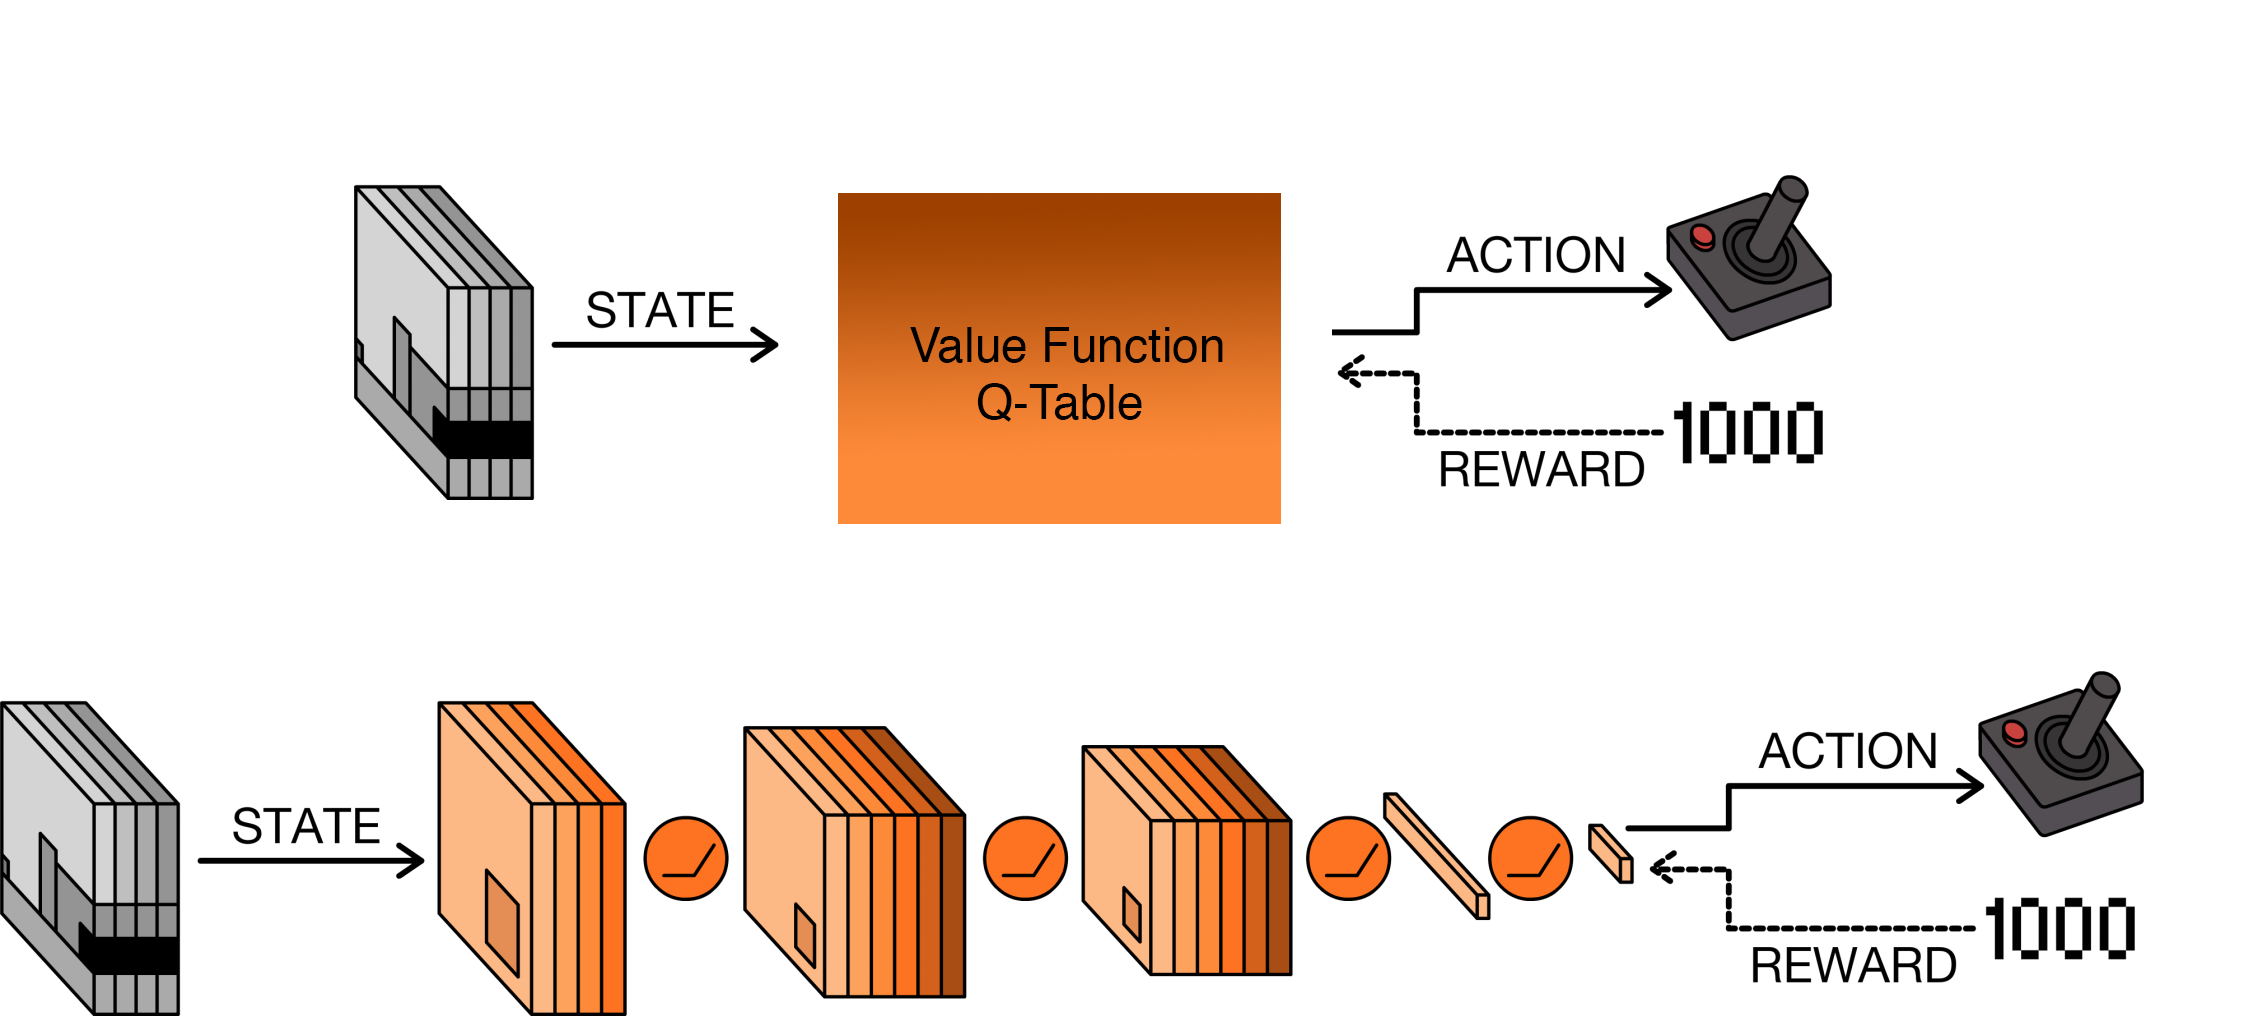
\includegraphics[width=0.95\linewidth ]{fig/dqn.png}
    \vspace{-2mm}
    \caption{Q-learning RL (above) and DQN (below) \cite{mnih2015human}.}
    \label{fig:dqn}
\end{figure}

\subsection{Current Research Challenges:}
To end with the short review on DRL, I present some of the research challenges in Deep Reinforcement Learning process.
\paragraph{Exploration vs Exploitation:}
Online decision making involves a fundamental choice {\em (i) Exploitation} or {\em (ii) Exploration}. Exploitation refers to making the best decision with the current information gathered by the agent. Whereas exploration involves attempting new action for more information. This is also known as {\em exploitation-exploration} dilemma. The best long-term strategy may involve lot of exploration and short term sacrifices. On the other hand if the agent has already found best strategy exploration, it may reduce the rewards.

\paragraph{Transfer Learning:}
Transfer learning is about efficiently using previous knowledge from a
source environment to achieve new (slightly) different tasks in a target environment. To achieve this, agent must develop generalization capabilities such as {\em (i) feature selection (ii) removing asymptotic bias (iii) reduce overfitting and function approximator (iv) Optimizing horizon} (length of observations history involved in decision making process) etc.

\paragraph{Learning without explicit reward function:}
In reinforcement learning, the reward function defines the goals to
be achieved by the agent. Due to the complexity of the environments in practical
applications, defining a reward function can turn out to be rather
complicated. Approaches like {\em imitation learning} (supervised learning) and {\em inverse reinforcement learning} where agent determines possible reward functions given observations of optimal behavior, are research challenges for the next decade.





%%% Local Variables:
%%% mode: latex
%%% TeX-master: "main"
%%% End:

\section{Part B.  Self Instructing Database:}
\label{part_b}
\subsection{Overview:}
Any standard database has considerable large number of configuration knobs. Databases needs to be tweaked with proper configuration for running efficiently with different workloads and hardware resources. Tweaking database configuration knobs needs a great level of expertise from database administrator (DBA) because optimal configuration varies with the type of workloads. Beside that, even finding optimal knob configurations might involve a trial and error process for a DBA (which restrits the search spaces for knobs). An auto-configuring database system or self intructing database is a desirable feature to demand from database companies.


Human database administrators rely on experience and intuition to configure it. DRL process mimick same learning strategies i.e. learn from mistakes and correctness to maximize future rewards. Keeping this in mind we can explore how DRL can provide a solution to automatic database tuning.


\subsection{Problem Formulation:}
Given a workload $\mathcal{W}$ (which is a serialized query profile DAG of execution task), with a knobs setting $\mathcal{C} = \{c_1,c_2,\ldots,c_{|\mathcal{C}|}\}$ a typical database outputs a log of metrics $\mathcal{M} = \{m_1,m_2,m_3,\ldots,m_{|\mathcal{M}|}\}$ as shown in Figure \ref{fig:database_01}.
The database keeps receiving workloads at some discrete interval of time and it runs with some configuration and outputs a metric log, which is also called a discrete time stochastic control process.

\begin{figure}[h]
	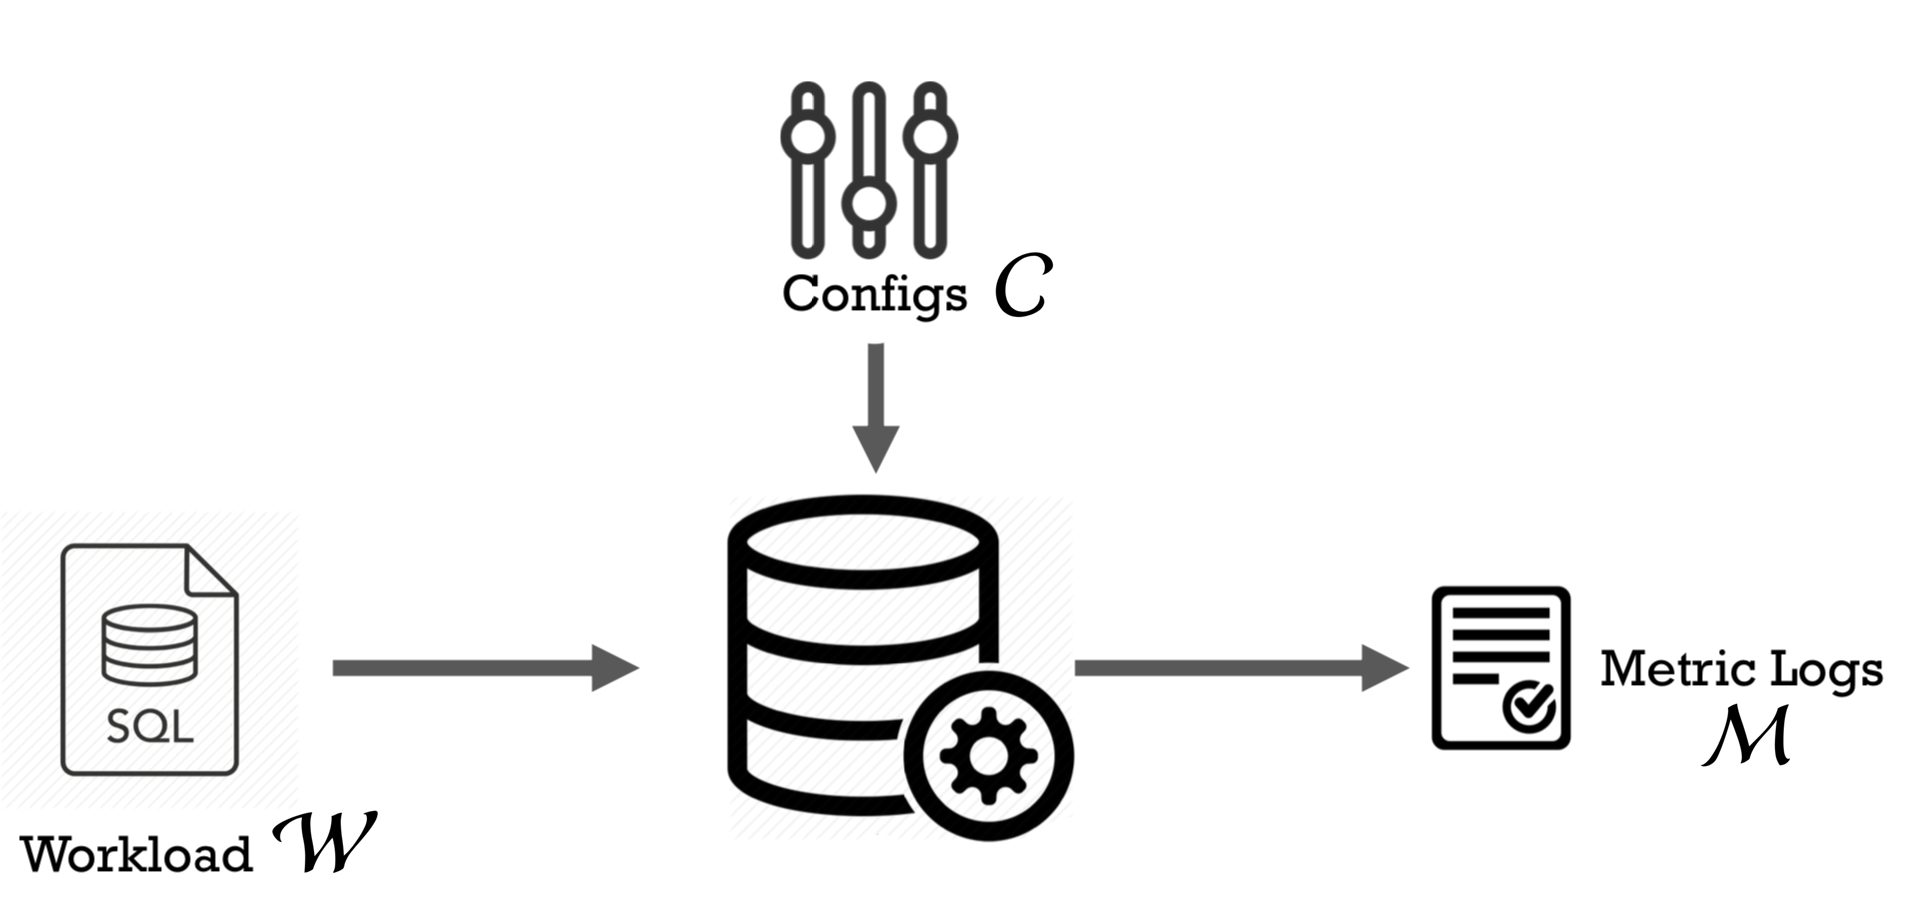
\includegraphics[width=0.9\linewidth ]{fig/database_01.png}
    \vspace{-2mm}
    \caption{A typical database system.}
    \label{fig:database_01}
\end{figure}


We can apply deep reinforcement learning to train a neural network in taking
over the database tuning process by optimizing configuration for observable database workload.
Essentially, we have to define a RL problem environment
consisting of the four following components to perform the learning as shown in Figure \ref{fig:database_agent}:


\textbf{1) Observable State:} This is also input to the neural network. This is typically the current workload in form of
query characteristics, for which the system should be optimised as well as the current state
of the configuration. Figure \ref{fig:database_agent} illustrates workload $\mathcal{W}_t$ is mapped to observation/state $\omega_t \in \Omega$ or $s_t \in  \mathcal{S}$ for time stamp $t$. (Note: $\omega_t = s_t$ in MPD)\\
\textit(Note: These notations are defined in Section \ref{formal_rl}).

\textbf{2) Actions:} An action is a bounded set of configuration $\mathcal{C}_t$ where each knobs can have a range of permissible values.
Changing the size of a database buffer is an example of action. Now we can represent $\mathcal{C}_t  \rightarrow a_t \in \mathcal{A}$.

\textbf{3) Reward:}
We map the metric $\mathcal{M}_t$ to rewards $r_t \in \mathcal{R}$. Since reward is a scalar function and metric $\mathcal{M}_t$ is a set of values representing the goodness and badness of database execution on workload $\mathcal{W}_t$, we need to apply some function $r_t = f(\mathcal{M}_t)$ to keep it simple. Later we will see an alternative approach where function $f$ is not needed with a mutitask-agent DRL.

\textbf{4) Hyperparamters for Neural Network:}
This includes properties of
the neural network (e.g. number of hidden layers, number of nodes per layer) as well as
properties of the learning process like the number of iterations.




% We apply this process into a RL agent-database environment interaction process as shown in Figure \ref{fig:database_agent}.
% In this process, at each time step $t$ we map metric $\mathcal{M}_t$ to rewards $r_t$. Similarly, workload $\mathcal{W}_t$ is mapped to observation/state $\omega_t$ or $s_t$, and configuration $C_t$ is mapped to action $a_t$.



\begin{figure}[h]
  \vspace{-3mm}
	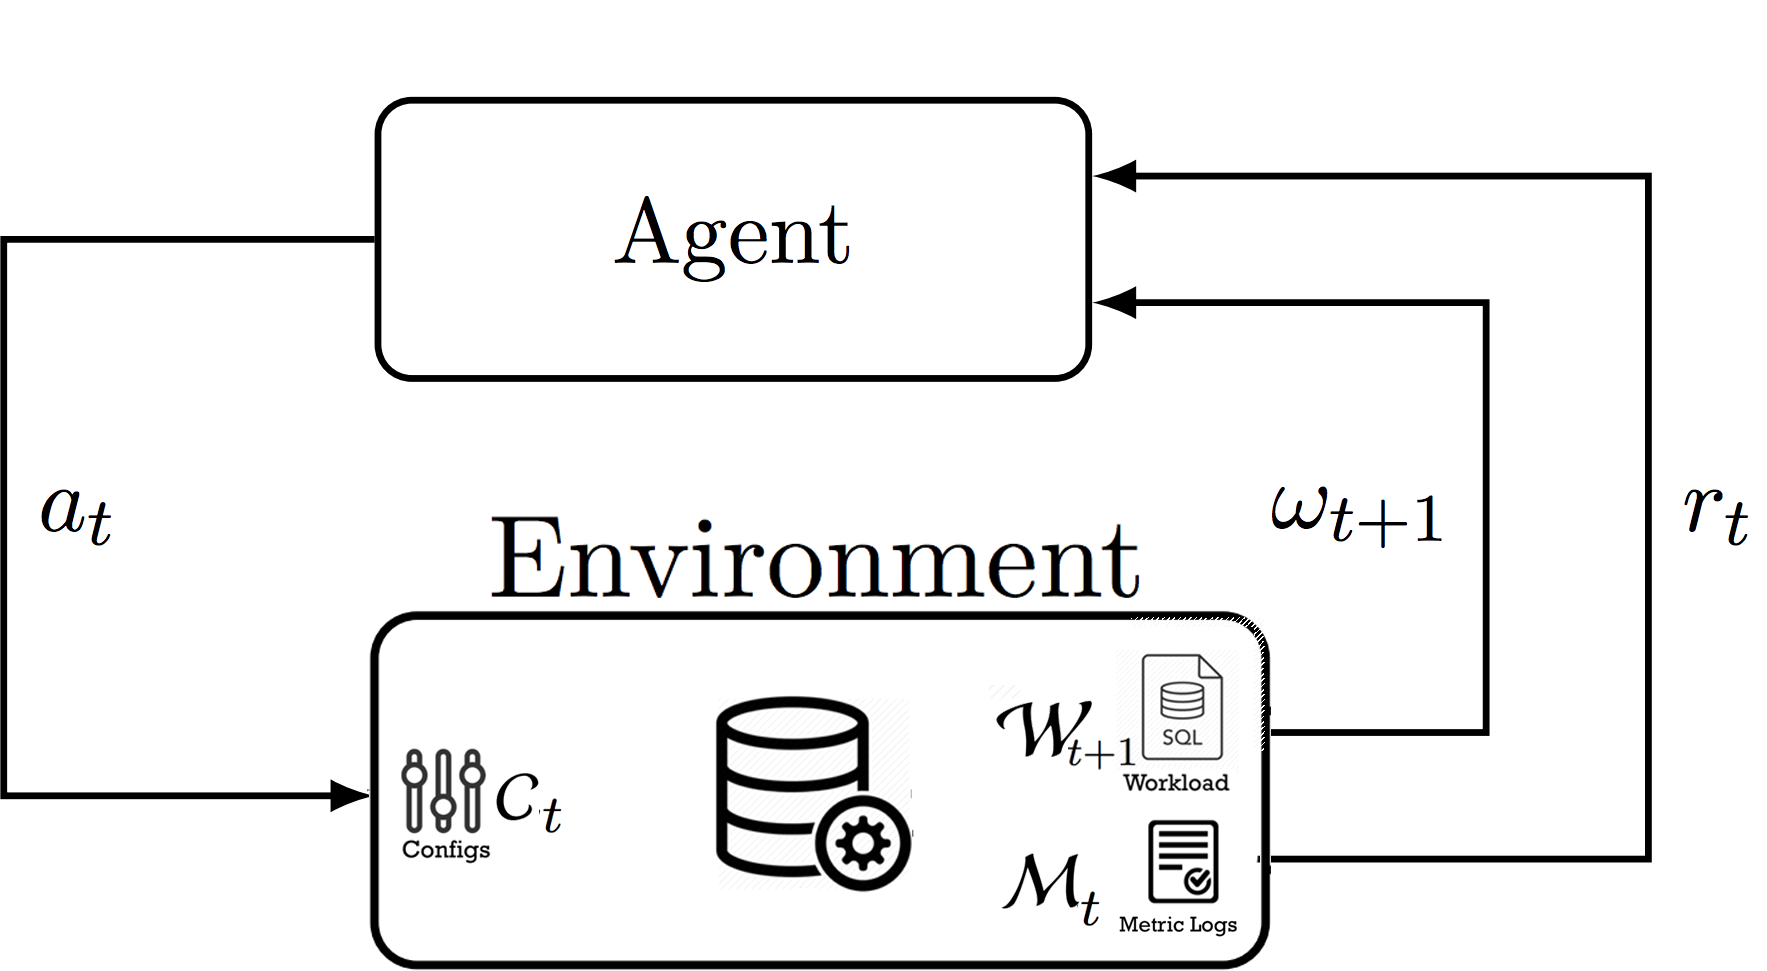
\includegraphics[width=\linewidth ]{fig/database_agent.png}
    \vspace{-5mm}
    \caption{RL Agent-Database Environment Interaction.}
    \label{fig:database_agent}
    \vspace{-5mm}
\end{figure}


\subsection*{Training and Challenges:}
With the high level components defined, now we will go through the workflow of learner.
Assuming the {\em neural network agent (NNA) } is configured with the required hyperparamters, the learning process starts with time $t=0$.
First, a workload $\mathcal{W}_t = s_t$  is fed into {\em neural network agent} (NNA). Then, the NNA explore action set $\mathcal{A}$ to produce an action (configuration) $a_t = \mathcal{C}_t$. The database environment on receiving action configuration $\mathcal{C}_t$ executes workload $\mathcal{W}_t$ and returns with metrics $\mathcal{M}_t$. Some function $f: \mathcal{M}_t \rightarrow r_t \in \mathbb{R}$ converts metric to scalar reward. This process is repeated many times and agents either explore action set or exploit learned optimal action to predict next best configuration. The desired goal is to optimize maximum cumulative positive rewards.

An intuitive solution for choosing function $f: \mathcal{M}_t \rightarrow r_t \in \mathbb{R}$ is  through the following steps:\\
\vspace{-4mm}
\begin{itemize}
  \item[-] negate all the metrics whose desired objective is to minimize, such that we now optimize, for maximization.
  \item[-] normalize each metric $m_i \in \mathcal{M}_t$ with their satisfied range of operation.
  \item[-] rewards is sum  of normalized metrics.
\end{itemize}

To avoid the problem of choosing a function $f$, we can transform the problem to a {\em Multi-task Deep RL} problem.
Some hierarchical RL techniques also decompose tasks into subtasks, these methods then solve the subtasks
in a locally optimal way and then global optimality can be achieved by aggregating back together. Another approach is to try {\em Linear Temporal Logic} specification that enables an interleaving of subtasks to support global optimization \cite{icarte2018teaching}.
These techniques can help in avoiding selection of $f$ by considering a specific set of metrics and optimize actions for it.


\paragraph{Model based/Model-free Agent:}
Model-free and model based both type of agent can be frutiful in this type of scenario. However model based approach needs more effort in design.
The advantage of model based approach is that it can learn strategies to trade-off exploration and eploitation to learn quickly.
But it is non-arguably plausible to choose gradient based methods because configurations knobs tend to have convex properties.
Also selecting RL agent components such as {\em value functions, policy functions, actor-critic or model} is subjected to further experimentation with various hyperparameters (such as number of hidden layers, ReLU layers etc.).

\paragraph{Transfer Learning:}
It is essential for this type of system that a learned agent adapt to a new environment or a new database.
Transfer learning is only possible when the agent can obtain generalization in learning procedure.
When the quality
of the dataset increases, the risk of overfitting is lower and the learning
algorithm can trust more the maximum likelihood model by looking
into a larger policy class and less approximations.
On the other hand, when the quality of the dataset is low, the learning algorithm should be
cautious on being too confident about the maximum likelihood model
and should favor more robust policies. Hence, the sampling technique to obtain a good coverage of sample space is important.


\subsection{Conclusion:}
In Section \ref{part_b} I presented an overview of the DRL model for autonomous or self-instructing databases. The model proposed is the starting point which can be extended as required for experimentation.  Challenges remaining have also been address in this small review.
A detailed deep dive with workload characteristics/representation is needed independently for future work on autonomous databases.








%%% Local Variables:
%%% mode: latex
%%% TeX-master: "main"
%%% End:


%\balance
%\vspace{-3mm}
\bibliographystyle{abbrv}
\bibliography{main}


% \vspace{-3mm}
% \bibliographystyle{ACM-Reference-Format}
% \bibliography{sigproc}

\end{document}
